\section{Wzroce projektowe (2) - strukturalne}

Strukturalne wzorce projektowe wyjaśniają jak łączyć obiekty i klasy z większe struktury zachowując jednocześnie prostotę i elastyczność.

\subsection{Adapter (ang. adapter)}

Wzorcem który pozwala na działanie dwóch komponentów o niezgodnych interfejsach nazywany jest Adapterem. Jeśli klasa potrzebuje do działania obiektu klasy o określonym interfejsie, natomiast klasa która mogłaby zostać wykorzystana posiada inny, niezgodny interfejs można utworzyć klasę adaptera, która dostosuje niezgodne interfejsy. Jest on stosowany do zmieniania interfejsu istniejącego kodu.

\begin{figure}[hbt!]
	\centering
	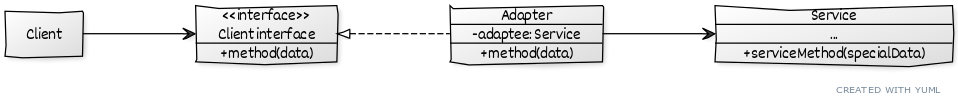
\includegraphics[width=0.9\linewidth]{images/AdapterUml}
	\caption{Diagram UML wzorca Adapter.}
	\label{lab3/fig/AdapterUml}
\end{figure}
%[Client interface]^-.-[Adapter]
%[Adapter]->[Service]
%[Client]->[Client interface]
%
%[Client]
%[<<interface>>Client interface|+method(data)]
%[Adapter|-adaptee: Service|+method(data)]
%[Service|...|+serviceMethod(specialData)]

Wyobraźmy sobie sytuację, w której mamy działający komponent i np. do logowania informacji o swoim działaniu wykorzystuje napisany przez nas zestaw. Klasa logera implementuje określony interfejs i przez ten interfejs klasa kliencka wykorzystuje zestaw do logowania. Jeśli za jakiś czas okażę się konieczne wykorzystanie bardziej rozbudowanego narzędzia np. pakietu NLog, możemy albo zmieniać odwołania w całym kodzie klienckim, albo wykorzystać adapter. W tym przypadku adapterem będzie klasa implementująca interfejs np. \texttt{ILogger} i posiadająca obiekt typu \texttt{NLog.Logger} przekazany np. jako argument konstruktora. Wszystkie metody interfejsu \texttt{ILogger} są przekazywane do odpowiednich metod pakietu \texttt{NLog}. Po napisaniu adaptera wystarczy wstrzyknąć nowo utworzony obiekt do kodu klienckiego bez dodatkowych modyfikacji. Nie będzie również problemem napisać dodatkowy adapter dla innego pakietu np. Log4N. Ze względu na fakt, że oba adaptery implementują ten sam interfejs można posiadać wiele różnych adapterów dla adaptowanych obiektów.

%https://stackoverflow.com/questions/9892137/windsor-pulling-transient-objects-from-the-container/9915056#9915056
% Steven answer
%Należy mieć na względzie, że dobrze jest logować informacje w możliwie jak najmniejszej liczbie miejsc. Często warto jest stworzyć blok \texttt{try{}catch{}} na samym szczycie aplikacji i to w tym miejscu przechwytywać wszystkie wyjątki.

%https://docs.microsoft.com/en-us/aspnet/core/fundamentals/logging/?view=aspnetcore-5.0#console
%https://codewithmukesh.com/blog/logging-with-nlog-in-aspnet-core/
%https://stackoverflow.com/questions/5646820/logger-wrapper-best-practice
%https://stackoverflow.com/questions/41243485/simple-injector-register-iloggert-by-using-iloggerfactory-createloggert/41244169#41244169
%https://blog.stephencleary.com/2018/06/microsoft-extensions-logging-part-2-types.html

% Why use generic version of ILogger over non-generic one
%Quoting Steven's comments on this question: "Injection of a ILogger<T> is just noise to the consumer that can lead to accidental errors when a wrong T is specified and it complicates testing."... "Injecting ILoggerFactory and ILogger<T> is a terrible idea, and as I see it, the only reason Microsoft is doing this (and promoting it publicly) is because their built-in container lacks the possibility to map a non-generic interface to a generic implementation." – Hooman Bahreini Nov 26 '20 at 22:22

Innym przykładem może być sytuacja w której posiadamy aplikację pobierająca dane z plików tekstowych w formacie \texttt{XML} i następnie je przetwarzającą oraz wizualizującą te dane w formie wykresów. Z czasem jednak może pojawić się potrzeba, aby dane pobierać z zewnętrznego serwera w formacie \texttt{JSON} korzystając z gotowego zestawu. Jeśli korzystamy z rozwiązań innych firm nie ma możliwość zmiany interfejsu zestawu pobierającego dane z serwera. Implementując wykorzystywany wcześniej interfejs możemy przekierowywać żądania od klienta do zewnętrznego zestawu w locie zmieniając format danych z \texttt{XML} na \texttt{JSON}.

Opisana powyżej wersja adaptera jest wersją obiektową tego wzorca. Można się również spotkać z podejściem klasowym, wtedy obiekt adaptera zamiast posiadać adaptowany obiekt, może po nim dziedziczyć. Jednak zgodnie z zasadą, aby przekładać kompozycję nad dziedziczenie ten wariant jest rzadziej stosowany. 

% Plusem adaptera klasowego jest możliwość przesłonięcia składowych wirtualnych, abstrakcyjnych. 
% W przypadku C++ stosując adapter klasowy należy publicznie dziedziczyć po klasie Target oraz prywatnie po klasie Adaptee.
% Podejście obiektowe jednak pozwala na działanie jednej kalsy Adapter z wieloma Adaptee

\subsubsection{Zadanie 1}
Celem tego zadania, będzie napisanie adaptera dla pakietu służącego do logowania informacji diagnostycznych w naszej aplikacji. Wykorzystany zostanie popularny pakiet NLog, który umożliwia bogaty zbiór sposobów logowania m.in. komunikaty mogą być wyświetlane na ekranie konsoli, wysyłane mailem, zapisywane do pliku, bazy danych, czy chmury. Zastosowanie adaptera pozwoli nam na wykorzystanie tego pakietu, bez konieczności uzależniana się od niego. Jeśli w przyszłości konieczne okaże się użycie np. Log4N zamiana będzie bardzo prosta.  

W pierwszej kolejności utwórz projekt aplikacji konsolowej .NET 5.0. Za pomocą menedżera pakietów dodaj pakiet NLog. Konfiguracja pakietu odbywa się z użyciem pliku NLog.config. Utwórz plik o takiej nazwie i~rozszerzaniu w~folderze projektu. Skopiuj do niego poniższe reguły logowania:
\begin{lstlisting}[caption={Konfiguracja pakietu NLog}, label={lab3/lst/nlogConfig}]
<?xml version="1.0" encoding="utf-8" ?>
<nlog xmlns="http://www.nlog-project.org/schemas/NLog.xsd"
	xmlns:xsi="http://www.w3.org/2001/XMLSchema-instance">

	<targets>
		<target name="logfile" xsi:type="File" fileName="logs.txt" />
		<target name="logconsole" xsi:type="Console" />
	</targets>

	<rules>
		<logger name="*" minlevel="Info" writeTo="logconsole" />
		<logger name="*" minlevel="Debug" writeTo="logfile" />
	</rules>
</nlog>
\end{lstlisting}
Plik zawiera targety oraz reguły. Te pierwsze wskazują, gdzie chcemy zapisać informacje, w tym przypadku na ekranie konsoli oraz w pliku tekstowym\footnote{Targety pakietu NLog moją bardzo bogate możliwości parametryzacji. Szczegóły można znaleźć na wiki repozytorium pakietu: \url{https://github.com/nlog/NLog/wiki}}. Reguły natomiast definiują jaki poziom ,,ważności'' informacji ma gdzie zostać przekierowany. Aby plik NLog.config mógł zostać wykorzystany konieczne jest jego przekopiowanie do folderu w plikiem wykonywalnym. Klikając PPM na nazwę pliku należy wybrać Properties i dalej w opcji Copy to Output Directory wskazać opcję Copy always.

Sprawdzić działanie pakietu można pobierając instancję logera metodą \texttt{GetCurrentClassLogger()}:
\begin{lstlisting}[caption={Wywołanie metod logujących pakietu NLog}, label={lab3/lst/nlogPackageTest}]
using NLog;

namespace AdapterDesignPattern
{
	class Program
	{
		private static readonly Logger Logger = LogManager.GetCurrentClassLogger();
		
		static void Main()
		{
			Logger.Info("Hello world");
			Logger.Error("Goodbye cruel world!");
		}
	}
}
\end{lstlisting}


Załóżmy, że nasza aplikacja wymaga wykorzystania narzędzia logującego. W tym celu będziemy wykorzystywać interfejs \texttt{ILogger}. Będzie on deklarował następującego metody typu \texttt{void} i przyjmującego argument typu \texttt{string}:
\begin{itemize}
	\item LogTrace
	\item LogDebug
	\item LogInformation
	\item LogWarning
	\item LogError
	\item LogCritical
\end{itemize}
Stwórz plik z powyższym interfejsem w osobnym pliku w projekcie. 

Dodaj do projektu prostą klasę, która w konstruktorze będzie oczekiwać obiektu implementującego utworzony przed chwila interfejs \texttt{ILogger}. Np.:
\begin{lstlisting}[caption={Przykład klasy wykorzystującej obiekt implementujący \texttt{ILogger}}, label={lab3/lst/customControllerWithLogger}]
public class CustomController
{
	private readonly ILogger logger;
	public CustomController(ILogger logger) => this.logger = logger;
	public void Get() => logger.LogInformation("Requested API");
}
\end{lstlisting}

Nie możemy przekazać logera NLog do obiektu typu \texttt{CustomController} ze względu na niezgodne interfejsy. Aby je dopasować wykorzystamy wzorzec projektowy Adapter. Dodaj do projektu klasę \texttt{NLogAdapter}. Zgodnie z diagramem UML\ref{lab3/fig/AdapterUml} klasa musi posiadać referencję do obiektu, który adaptuje. W tym przypadku będzie to klasa \texttt{Logger} pakietu NLog. W klasie adaptera dodaj konstruktor z parametrem typu \texttt{NLog.Logger}. Dodatkowo klasa powinna implementować interfejs \texttt{ILogger}. Zaimplementuj metody deklarowane przez ten interfejs\footnote{Wszystkie wymagane składowe można łatwo umieścić w klasie poprzez najechanie myszką na nazwę interfejsu (powinna być podkreślona czerwonym kolorem) i kliknięcie ,,Show potential fixes'' (albo skrótem Alt+Enter) i wybranie opcji ,,Implement interface''}, w taki sposób aby przekierowywały wywoływania metod to metod obiektu \texttt{NLog.Logger} np. w~taki sposób:
\begin{lstlisting}[caption={Fragment klasy adaptera dla pakietu NLog}, label={lab3/lst/nlogAdapter}]
 public class NLogAdapter : ILogger
{
	private readonly NLog.Logger logger;	
	public NLogAdapter(NLog.Logger logger) => this.logger = logger;	
	public void LogDebug(string message) => this.logger.Debug(message);	
	//...
}
\end{lstlisting}

Teraz usuń z metody \texttt{Main} napisane wcześniej sprawdzenie poprawności działania pakietu NLog i~utwórz instancję klasy \texttt{CustomController}. Jako argument przekaż obiekt \texttt{NLogAdapter}. Wywołaj metodę \texttt{Get()} klasy \texttt{CustomController} i sprawdź czy log pojawił się na ekranie konsoli oraz w pliku tekstowym \texttt{logs.txt}.


\subsection{Kompozyt (ang. composite)}

Kompozyt łączy obiekty w struktury drzewiaste i pozwala klientom traktować je jak osobne obiekty. Drzewo składa się z dwóch rodzajów elementów liści oraz kontenerów. Kontener może składać się z liści oraz z innych kontenerów. Wzorzec ten powinien być stosowany jeżeli z punktu widzenia klienta nie ma znaczenia czy odwołuje się on do pojedynczego elementu czy drzewiastej struktury. Zazwyczaj klient nie wie z jakiego typu elementu korzysta. Klient będzie ignorował różnice pomiędzy pojedynczymi, a złożonymi obiektami.


Dodatkowo istnieje możliwość dodania nowych typów, które mogą być liśćmi drzewa bez zmiany kodu klienta. Jest to właściwość zgodna z zasadą otwarte/zamknięte. Trudne może okazać się znalezienie wspólnego interfejsu dla wszystkim elementów Kompozytu. Do tworzenia drzew kompozytowych często korzysta się z wzorca Budowniczy.

Wzorzec Kompozyt wykorzystuje interfejs albo klasę abstrakcyjną do reprezentacji zarówno typów prostych jak i złożonych. Wszystkie one muszą implementować wspólny interfejs albo dziedziczyć po klasie abstrakcyjnej.
 
\begin{figure}[hbt!]
	\centering
	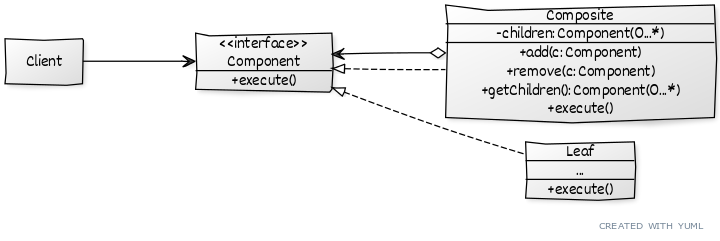
\includegraphics[width=0.8\linewidth]{images/CompositeUml}
	\caption{Diagram UML wzorca kompozyt.}
	\label{lab3/fig/CompositeUml}
\end{figure}
%[Client]->[Component]
%[Component]^-.-[Composite]
%[Composite]<>->[Component]
%[Component]^-.-[Leaf]
%
%[Client]
%[<<interface>>Component|+execute()]
%[Leaf|...|+execute()]
%[Composite|-children: Component(0...*)|+add(c: Component);+remove(c: Component);+getChildren(): Component(0...*);+execute()]

Łatwo można sobie wyobraź drzewo składające się z produktów oraz pudełek (kontenerów) które je przechowują. Zarówno liście jak i kontenery implementują wspólny interfejs. Klient wywołuję metodę np. \texttt{GetPrice()} głównego kontenera (korzenia). Jeśli dzieckiem danego wierzchołka jest liść (produkt ) zwracana jest jego cena, żądanie zostaje obsłużone bezpośrednio. Jeśli natomiast dzieckiem jest inny kontener (obiekt \texttt{Composite}) to przeglądana jest jego zawartość i ponownie w zależności od zawartości podejmowana jest akcja dalszego przeglądania albo zwracania wartości ceny.

Interfejsy graficzne, systemy SCADA zwykle pozwalają na rysowanie złożonych elementów z wielu prostych elementów. Klient nie chce traktować prostych i złożonych elementów w odmienny sposób. Powoduje do dodatkowe skomplikowanie modułu programu. Klasy \texttt{Line}, \texttt{Rectangle}, \texttt{Text} definiują proste elementy graficzne. Natomiast klasa \texttt{Picture} mogłaby stanowić kontener, w którym były przechowywane proste elementy podrzędne.

\subsubsection{Zadanie 2}

Utwórz nowy projekt (aplikację konsolową .NET 5). Dodaj w nim folder o nazwie \texttt{Equipments}. Wewnątrz tego folderu dodaj klasę abstrakcyjną komponentu \texttt{Equipment}\ref{lab3/lst/compositeAbstractClass}. Definiuje ona wspólny dla wszystkich klas interfejs. To po niej będą dziedziczyły klasy liści oraz kompozytów (kontenerów). Struktura drzewiasta będzie zawierała elementy komputera PC. Będzie posiadała kontenery np. płytę główną, która może dalej zawierać proces oraz pamięć RAM, którą są liśćmi.
\begin{lstlisting}[caption={Przykład abstrakcyjnej klasy komponentu}, label={lab3/lst/compositeAbstractClass}]
	abstract class Equipment
	{
		public abstract decimal NetPrice();
		public abstract decimal DiscountPrice();	
		public abstract int Power();
		public virtual void Add(Equipment component) => throw new NotImplementedException();	
		public virtual void Remove(Equipment component) => throw new NotImplementedException();
		public virtual bool IsComposite() => true;
	}
\end{lstlisting}
%Normlanie lepiej byłoby zamiast stosować podstawowe typu utworzyć klasę Currency.
Następnie w tym samym folderze dodaj kolejne klasy zarówno kontenerów np. \texttt{Chasis} oraz \texttt{Motherboard} oraz liści np. \texttt{Cpu}, \texttt{FloppyDisk}. Wszystkie powinny dziedziczyć po klasie \texttt{Equipment}. Przykładowa implementacja klasy \texttt{FloppyDisk} może być następująca:
\begin{lstlisting}[caption={Przykład klasy będącej liściem kompozytu}, label={lab3/lst/compositeLeafFloppyDisk}]
class FloppyDisk : Equipment
{
	private readonly decimal price;
	private readonly decimal discount;
	private readonly int power;
	
	public FloppyDisk(decimal price, decimal discount, int power)
	{
		this.price = price;
		this.discount = discount;
		this.power = power;
	}

	public override decimal NetPrice() => price;	
	public override bool IsComposite() => false;	
	public override decimal DiscountPrice() => price * (1 - discount);
	public override int Power() => power;
}
\end{lstlisting}
Klasa kontenera dodatkowo powinna posiadać pole listy na inne kontenery i liście oraz implementować metody wirtualne \texttt{Add} i \texttt{Remove}. Natomiast metody \texttt{NetPrice}, \texttt{DiscountPrice} oraz \texttt{Power} muszą przeglądać dodane wcześniej komponenty (liście lub inne kontenery) i zwracać sumę wszystkich wartości.
\begin{lstlisting}
class MotherBoardEquipment : Equipment
{
	protected List<Equipment> equipments = new List<Equipment>();

	//...
		
	public override void Add(Equipment component) => equipments.Add(component);	
	public override void Remove(Equipment component) => equipments.Remove(component);
	public override decimal NetPrice()
	{
		decimal result = price;
		equipments.ForEach(x => result += x.NetPrice());	
		return result;
	}
		
	//...
}
\end{lstlisting}

W klasie klienta, albo w metodzie \texttt{Main} sprawdź poprawność stworzonej struktury. Utwórz obiekt obudowy (\texttt{ChasisEquipment}) oraz dodaj do niego (za pomocą metody \texttt{Add}) kilka dysków twardych \texttt{FloppyDisk} oraz płytę główną \texttt{MotherBoardEquipment} do której wcześniej dodaj procesor \texttt{Cpu}.

Tak utworzoną strukturę możesz teraz przekazać do innej klasy, która może z tej całej struktury korzystać tak jak z pojedynczego obiektu nie zdając sobie sprawy z implementacji i jej złożoności.
\begin{lstlisting}
class Client
{
	public void PrintBill(Equipment equipment)
	{
		Console.WriteLine($"Bill:\n\t{equipment.NetPrice()}\n\t{equipment.DiscountPrice()}\n\t{equipment.Power()}");
	}
}
\end{lstlisting}

\subsection{Fasada (ang. facade)}
Jeśli istnieje potrzeba, aby ukryć złożoność biblioteki albo innego zbioru wielu klas można użyć wzorca fasady. Jest to bardzo prosty wzorzec upraszczający sposób w jaki klienci korzystają z współpracujących, zależnych od siebie klas. Udostępnia ona jednolity interfejs dla zbioru interfejsów z podsystemu. Wykorzystując fasadę klient nie musi tworzyć, ani zarządzać zależnościami pomiędzy obiektami są one przed nim ukryte za interfejsem fasady. Fasada może również służyć za punkt wejścia dla podsystemu w~warstwowo podzielonym zestawie.

Fasada pozwala zmniejszyć liczbę obiektów z której korzystają klienci. Dodatkowo wprowadza się luźne powiązanie pomiędzy klientami, a podsystemami. Ułatwione jest wprowadzanie zmian w podsystemach czy zmiana zależności między nimi. 

\begin{figure}[hbt!]
	\centering
	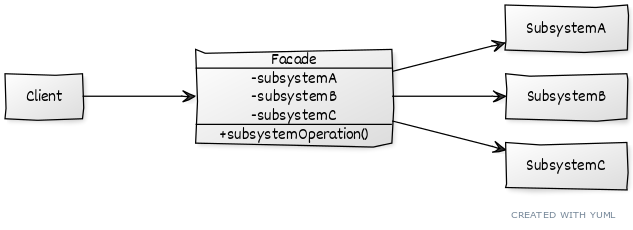
\includegraphics[width=0.8\linewidth]{images/FacadeUml}
	\caption{Diagram UML wzorca Fasada.}
	\label{lab3/fig/FacadeUml}
\end{figure}
%[Client]->[Facade]
%[Facade]->[SubsystemA]
%[Facade]->[SubsystemB]
%[Facade]->[SubsystemC]
%
%[Client]
%[Facade|-subsystemA;-subsystemB;-subsystemC|+subsystemOperation()]
%[SubsystemA]
%[SubsystemB]
%[SubsystemC]

Interfejs udostępniany przez omawiany wzorzec jest zazwyczaj uproszczony, nie posiada wszystkich funkcjonalności, które zapewniają ukrywane przez niego klasy. Dostarczane są jedynie te niezbędne. Jedynie bardziej wymagający klienci będą musieli spojrzeć za fasadę.

Przykładem zastosowania fasady może być proces konwersji materiału wideo. Jest on złożony, wykorzystuje różne klasy do kompresji materiału wideo, miksowania audio, zmiany formatu pliku itp. Klient może potrzebować jedynie uproszczonego interfejsu do konwertowania pliku wideo. Nie muszą go interesować złożone mechanizmy tego procesu. Dlatego zamiast zmuszać klienta do posiadania i zarządzania wieloma klasami, można utworzyć klasę fasady, która te złożoności ukryje. Jeśli w przyszłości część wykorzystywanych klas się zmieni, aktualizacja kodu będzie potrzebna tylko w jednym miejscu, w klasie fasady.

Innym przykładem może być podsystem kompilujący. Klienta nie interesują złożone zależności pomiędzy parserem, preprocesorem, analizatorem semantyki czy optymalizatorem. Autorzy klientów chcą tylko skompilować kod. Jeśli proces kompilacji zostanie ukryty w~pojedynczej klasie \texttt{Compiler}, bo będzie ona odgrywała właśnie rolę fasady. Będzie ona udostępniać klientom prosty interfejs do kompilacji.
% g++ -Wall -std=c++14 main.cpp -o main.exe //-Wall (all warnings) and -o main.exe instead of a.exe

\subsubsection{Zadanie 3}

Utwórz kolejny projekt analogicznie jak poprzednio. Tym razem zostanie wykorzystany wzorzec projektowy Fasady do ukrycia złożoności serwisów odpowiedzialnych za pobieranie informacji o konkretnych parametrach pogody.

Dodaj do projektu folder \texttt{WeatherServices}. Następnie umieść w nim trzy interfejsy w osobnych plikach: \texttt{ITemperatureService}, \texttt{IHumidityService} oraz \texttt{IForecastService}. Każdy z nich niech deklaruje jedną metodę odpowiednio: \texttt{double GetTemperature()}, \texttt{double GetHumidity()} i \texttt{double GetForecast()}. 

Dodaj teraz do tego samego folderu trzy klasy implementujące te interfejsy. W celu wygenerowania pomiarów możesz skorzystać z~generatora liczb pseudolosowych z klasy \texttt{System.Radnom} i jej metody \texttt{NextDouble}. Generacja liczb z pewnego przedziału może być zrealizowana w następujący sposób:
\begin{lstlisting}	
	random.NextDouble() * (maxValue - minValue) + minValue;
\end{lstlisting}
Można również dodać tzw. metodę rozszerzającą (ang. Extension Method). Pozwala ona na ,,dodanie'' metody do już istniejącego typu, w tym przypadku \texttt{Random}, bez konieczności tworzenia nowej klasy pochodnej czy modyfikacji klasy już istniejącej. Metody rozszerzające są statyczne, ale ich wywołanie wygląda jakby należało do instancji danej klasy. Kompilator tłumaczy następnie wywołanie tej metody na metodę statyczną. 
% Enkapsulacja nie jest naruszona, metody rozszerzajace nie maja dostepu do składowych prywatnych.

Dodaj do osobnego folderu w projekcie o nazwie np. \texttt{Extensions} statyczną klasę \texttt{RandomExtension} w niej statyczną metodę w następującej postacji:
\begin{lstlisting}	
	public static class RandomExtensions
	{
		public static double NextDouble(
		this Random random,
		double minValue,
		double maxValue)
		{
			return random.NextDouble() * (maxValue - minValue) + minValue;
		}
	}
\end{lstlisting}
Zwróć uwagę na pierwszy parametr, określa on do jakiego typu (klasy) chcemy dodać nową metodę. Konieczne jest, aby poprzedzić go słowem kluczowym \texttt{this}. Kolejne parametry nie różnią się niczym od tych ze standardowej deklaracji metody.

Po dodaniu klasy \texttt{RadndomExtension} klasa \texttt{Random} ,,otrzymała'' nową metodę, która generuje liczbę pseudolosową typu \texttt{double} z określonego przez klienta przedziału. 

Metod rozszerzających nie należy stosować tam gdzie możemy modyfikować kod klasy, dodać składową. Jest to jednak dobre narzędzie jeśli chcemy dodać funkcjonalność do kodu, który nie jest pod naszą kontrolą, a dziedziczenie jest nieodpowiednie albo niemożliwe. 

%To generate a cryptographically secure random number, such as one that's suitable for creating a random password, use the RNGCryptoServiceProvider class or derive a class from System.Security.Cryptography.RandomNumberGenerator.

Klasa \texttt{TemperatureService} może teraz wyglądać następująco (zwróć uwagę na wykorzystanie wcześniej wspomnianej metody rozszerzającej):
\begin{lstlisting}	
public class TemperatureService : ITemperatureService
{
	public double GetTemperature()
	{
		var randomGenerator = new Random();
		return randomGenerator.NextDouble(-20, 40);
	}
}
\end{lstlisting}

Dalej w głównym katalogu projektu dodaj rekord \texttt{Weather} w osobnym pliku:
\begin{lstlisting}	
public record Weather(double Temperature, double Humidity, double Forecast);
\end{lstlisting}

Teraz umieść z katalogu głównym Fasadę (nową klasę) dla wcześniej stworzonych serwisów. Klasa Fasady niech zawiera trzy pola na obiekty implementujące utworzone interfejsy. W konstruktorze przypisz im przekazane przez parametry konstruktora obiekty. Dodaj również metodę \texttt{GetWeatherInformation} zwracającą obiekt typu \texttt{Weather}. Metoda ta niech pobiera informacje o temperaturze, wilgotności oraz estymacji z~serwisów i zwraca jeden obiekt zawierający te dane:
\begin{lstlisting}	
public class WeatherApiFasade
{
	//...
	
	public WeatherApiFasade(ITemperatureService temperatureService, 
		IHumidityService humidityService,
		IForecastService forecastService)
	{
		//...
	}
	
	public Weather GetWeatherInformation()
	{
		return  new(
			temperatureService.GetTemperature(),
			humidityService.GetHumidity(),
			forecastService.GetForecast());
	}
}
\end{lstlisting}

Na koniec dodaj klasę \texttt{Application}:
\begin{lstlisting}	
class Application
{
	public static void Run(WeatherApiFasade weatherApiFasade)
	{
		Console.Write(weatherApiFasade.GetWeatherInformation());
	}
}
\end{lstlisting}
oraz w metodzie \texttt{Main} utwórz obiekt typu \texttt{WeatherApiFasade} przekazując mu wcześniej utworzone obiekty wymagane przez konstruktor. Wywołaj metodę \texttt{Run()} i sprawdź czy na ekranie konsoli zostały wypisane oczekiwane wyniki:
\begin{lstlisting}	
static void Main(string[] args)
{
	WeatherApiFasade weatherApiFasade = new WeatherApiFasade(
		new TemperatureService(), 
		new HumidityService(),
		new ForecastService());
	
	Application.Run(weatherApiFasade);
}
\end{lstlisting}
